\documentclass[
10pt, % Main document font size
a4paper, % Paper type, use 'letterpaper' for US Letter paper
oneside, % One page layout (no page indentation)
%twoside, % Two page layout (page indentation for binding and different headers)
headinclude,footinclude, % Extra spacing for the header and footer
BCOR5mm, % Binding correction
]{scrartcl}
\usepackage{hyperref}
\usepackage{lettrine}
\usepackage{listings}
\usepackage{color}

\definecolor{dkgreen}{rgb}{0,0.6,0}
\definecolor{gray}{rgb}{0.5,0.5,0.5}
\definecolor{mauve}{rgb}{0.58,0,0.82}

\lstset{frame=tb,
  language=Java,
  aboveskip=3mm,
  belowskip=3mm,
  showstringspaces=false,
  columns=flexible,
  basicstyle={\small\ttfamily},
  numbers=none,
  numberstyle=\tiny\color{gray},
  keywordstyle=\color{blue},
  commentstyle=\color{dkgreen},
  stringstyle=\color{mauve},
  breaklines=true,
  breakatwhitespace=true,
  tabsize=3
}
%%%%%%%%%%%%%%%%%%%%%%%%%%%%%%%%%%%%%%%%%
% Arsclassica Article
% Structure Specification File
%
% This file has been downloaded from:
% http://www.LaTeXTemplates.com
%
% Original author:
% Lorenzo Pantieri (http://www.lorenzopantieri.net) with extensive modifications by:
% Vel (vel@latextemplates.com)
%
% License:
% CC BY-NC-SA 3.0 (http://creativecommons.org/licenses/by-nc-sa/3.0/)
%
%%%%%%%%%%%%%%%%%%%%%%%%%%%%%%%%%%%%%%%%%

%----------------------------------------------------------------------------------------
%	REQUIRED PACKAGES
%----------------------------------------------------------------------------------------

\usepackage[
nochapters, % Turn off chapters since this is an article        
beramono, % Use the Bera Mono font for monospaced text (\texttt)
eulermath,% Use the Euler font for mathematics
pdfspacing, % Makes use of pdftex’ letter spacing capabilities via the microtype package
dottedtoc % Dotted lines leading to the page numbers in the table of contents
]{classicthesis} % The layout is based on the Classic Thesis style

\usepackage{arsclassica} % Modifies the Classic Thesis package

\usepackage[T1]{fontenc} % Use 8-bit encoding that has 256 glyphs

\usepackage[utf8]{inputenc} % Required for including letters with accents

\usepackage{graphicx} % Required for including images
\graphicspath{{Figures/}} % Set the default folder for images

\usepackage{enumitem} % Required for manipulating the whitespace between and within lists

\usepackage{lipsum} % Used for inserting dummy 'Lorem ipsum' text into the template

\usepackage{subfig} % Required for creating figures with multiple parts (subfigures)

\usepackage{amsmath,amssymb,amsthm} % For including math equations, theorems, symbols, etc

\usepackage{varioref} % More descriptive referencing

%----------------------------------------------------------------------------------------
%	THEOREM STYLES
%---------------------------------------------------------------------------------------

\theoremstyle{definition} % Define theorem styles here based on the definition style (used for definitions and examples)
\newtheorem{definition}{Definition}

\theoremstyle{plain} % Define theorem styles here based on the plain style (used for theorems, lemmas, propositions)
\newtheorem{theorem}{Theorem}

\theoremstyle{remark} % Define theorem styles here based on the remark style (used for remarks and notes)

%----------------------------------------------------------------------------------------
%	HYPERLINKS
%---------------------------------------------------------------------------------------

\hypersetup{
%draft, % Uncomment to remove all links (useful for printing in black and white)
colorlinks=true, breaklinks=true, bookmarks=true,bookmarksnumbered,
urlcolor=webbrown, linkcolor=RoyalBlue, citecolor=webgreen, % Link colors
pdftitle={}, % PDF title
pdfauthor={\textcopyright}, % PDF Author
pdfsubject={}, % PDF Subject
pdfkeywords={}, % PDF Keywords
pdfcreator={pdfLaTeX}, % PDF Creator
pdfproducer={LaTeX with hyperref and ClassicThesis} % PDF producer
} 

\hyphenation{Fortran hy-phen-ation} 
\title{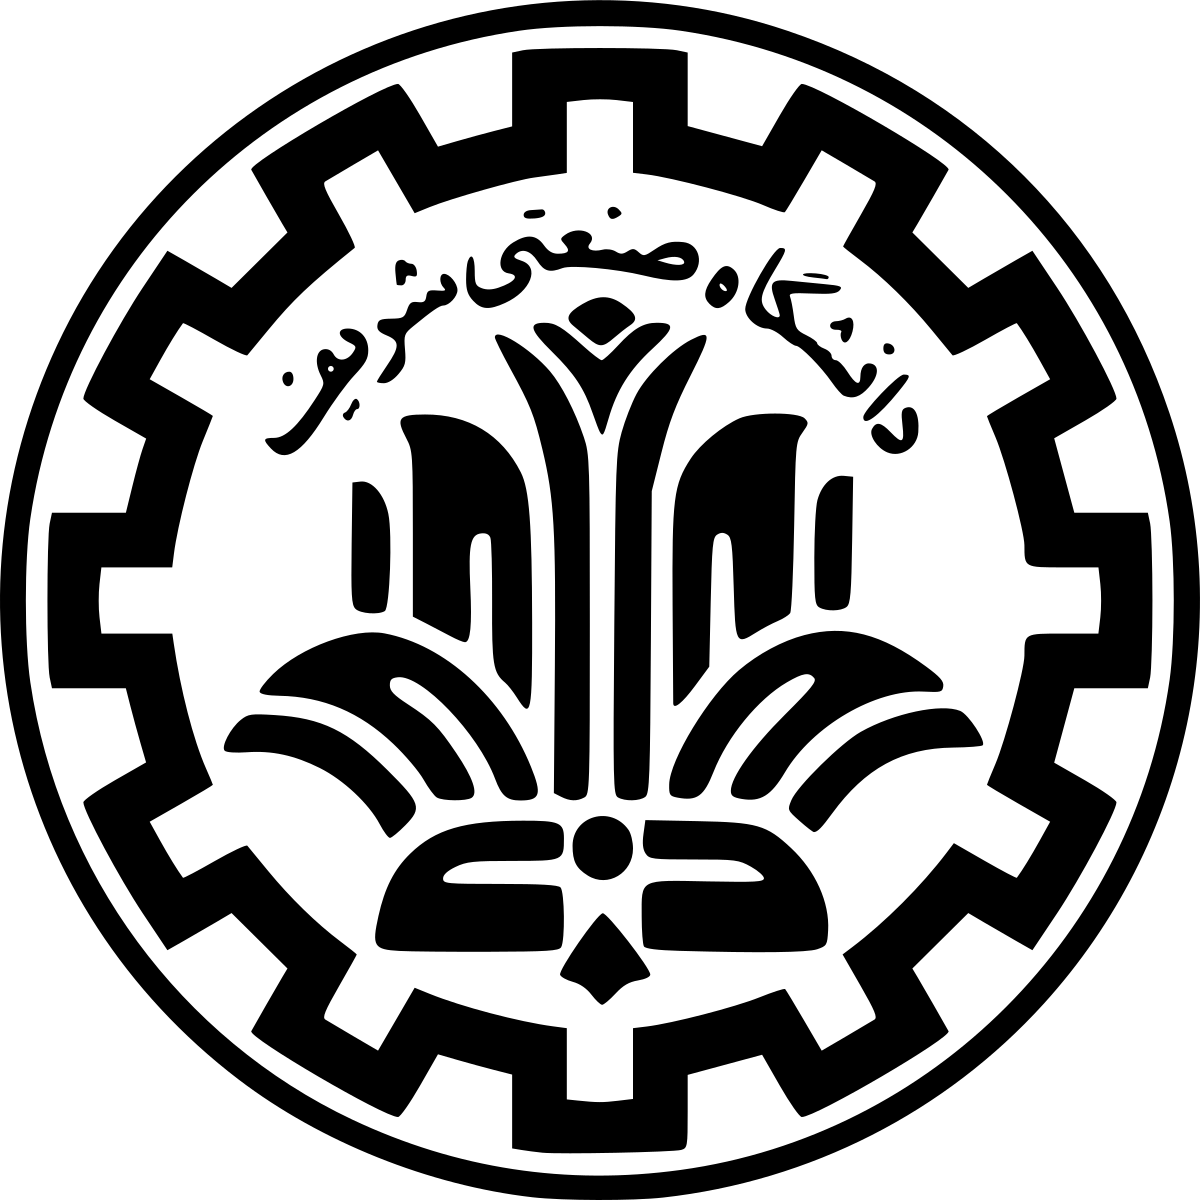
\includegraphics[scale=0.2]{Sharif-Logo.png}\\\normalfont\spacedallcaps{DETERMINING THE PROPER SORTING ALGORITHM BASED ON THE GIVEN DATA}}

\author{\spacedlowsmallcaps{Parham Houshmand, Yasamin Vaziri 
} \\
\spacedlowsmallcaps{Mahya Mottaghi \& Elham Soleimani}
}

\date{
\spacedlowsmallcaps{Sharif University of Technology}
\\
July 2022 }

\begin{document}


\renewcommand{\sectionmark}[1]{\markright{\spacedlowsmallcaps{#1}}} % The header for all pages (oneside) or for even pages (twoside)
%\renewcommand{\subsectionmark}[1]{\markright{\thesubsection~#1}} % Uncomment when using the twoside option - this modifies the header on odd pages
\lehead{\mbox{\llap{\small\thepage\kern1em\color{halfgray} \vline}\color{halfgray}\hspace{0.5em}\rightmark\hfil}} % The header style

\pagestyle{scrheadings} % Enable the headers specified in this block

%----------------------------------------------------------------------------------------
%	TABLE OF CONTENTS & LISTS OF FIGURES AND TABLES
%----------------------------------------------------------------------------------------

\maketitle % Print the title/author/date block

\setcounter{tocdepth}{2} % Set the depth of the table of contents to show sections and subsections only

\tableofcontents % Print the table of contents
\newpage
%\listoffigures % Print the list of figures

%\listoftables % Print the list of tables

%----------------------------------------------------------------------------------------
%	ABSTRACT
%----------------------------------------------------------------------------------------

\section{Abstract}
\lettrine[findent=2pt]{\textbf{T}}{ }he cost of using sorting algorithms may have a considerable difference in that finding the proper algorithm reduces time and space and improves sorting efficiency.
There are linear sorting algorithms that need to be preprocessed before they can be used.
The quick sort algorithm also needs the data to be unsorted and sometimes according to the structured data we have (heap, linked list) they need another special algorithm (heap and merge sort) also sometimes the data is very voluminous, and We have to use an algorithm that performs in place sorting. According to these interpretations, we perform linear pre-processing on the primary data to find the proper sorting algorithm with the features we mention from each sorting algorithm.
\begin{center}
 \emph{keywords}:algorithm, sorting, data, input, proper sorting algorithm, time complexity
\end{center}
 
\section{Introduction}

As there are different sorting algorithms, we know they have  
bold differences with each other and we are going to give a short summary about them. But the main reason of this paper is to construct the proper sorting algorithm with given input which has the minimum time complexity no matter what the size of input is.Our algorithm firstly checks each number behind the head whether it is ascending or descending, also checks whether the number is negative or not, then it finds the largest length of the number and the largest number, after that it checks its inversion and then it finds whether the inversion is larger than n$\log$ n or not. Note that for radix and count sort the ascending order should not neither be less than n$\log n$ nor negative.

\section{Methods}

inja zanak ax doos dare model konim ax nemoodar jadval.  comment gozari shode bashe.
tahlil azmayesham bayad benevisim (khoobia va badiaye algoritm khodemoon )
\begin{enumerate}[noitemsep]
\item different methods of sorting
\item different techniques
\item Analysis of sorting techniques 
\item proper sorting algorithm analysis
\end{enumerate}

%------------------------------------------------

\subsection{different sorts time complexity}

\paragraph{}  
\begin{enumerate}[noitemsep]
\item  Bubble sort and Insertion sort
\\
The average and worst case time complexity of both is $n^2 $ while the best time complexity is n. This happens when the array is already sorted, instead the worst case is when the array is completely reversed. 
and as a use, these algorithms work better for the smaller data and insertion sort is of order of n when the array is sorted.


\item Merge sort
\\
Merge sorts best, average and worst case time complexity is$nlogn$ and again similarly independent of distribution of data. for this algorithm we can say it works the best when the array is reversed sort

\item Heap sort
\\
like merge sort, its best, average and worst case time complexity is $nlogn$ which is independent of distribution of data. 
heap sort's property is that the space is of order of 1.
\item Quick sort
\\
It is a divide and conquer approach with recurrence relation: 
$$T(n) = T(k) + T(n-k-1) + cn$$
Its worst case is when the array is sorted or reverse sorted, the partition algorithm divides the array in two sub arrays with $0$ and $n-1$ elements. Therefore, 
$$T(n) = T(0) + T(n-1) + cn$$
Solving this we get:
$$T(n) = O(n^2)$$
On an average, the partition algorithm divides the array in two subarrays with
 equal size. Therefore,
$$T(n) = 2T(\frac{n}{2}) + cn$$
and finally
$$T(n) = O(nlogn)$$
the algorithm is of order of $n^2$ when the array is revered.
Non-comparison based sorting:
\\
In non-comparison based sorting, elements of array are not compared with each other to find the sorted array.
\\

\item Radix sort
\\
Best, average and worst case time complexity for radix sort is $nk$ where $k$ is the maximum number of digits in elements of array. 
\\

\item Count sort
\\
For this algorithm best, average and worst case time complexity is $n+k$ where k is the size of count array.



\end{enumerate}




%------------------------------------------------

\subsection{common techniques}
\begin{enumerate}[noitemsep]
\item in place \& out place technique
\\
A sorting technique is inplace if it does not use any extra memory to sort the array. 
Among the comparison based techniques discussed, only merge sort is outplaced technique as it requires an extra array to merge the sorted subarrays. 
Among the non-comparison based techniques discussed, all are outplaced techniques. Counting sort uses a counting array and bucket sort uses a hash table for sorting the array. 

\item online \& offline technique
\\
A sorting technique is considered Online if it can accept new data while the procedure is ongoing i.e. complete data is not required to start the sorting operation. 
Among the comparison based techniques discussed, only Insertion Sort qualifies for this because of the underlying algorithm it uses i.e. it processes the array (not just elements) from left to right and if new elements are added to the right, it doesn’t impact the ongoing operation. 

\item Stable \& unstable technique
\\
A sorting technique is stable if it does not change the order of elements with the same value. 
Out of comparison based techniques, bubble sort, insertion sort and merge sort are stable techniques. Selection sort is unstable as it may change the order of elements with the same value. For example, consider the array $4, 4, 1, 3.$ 
In the first iteration, the minimum element found is 1 and it is swapped with 4 at 0th position. Therefore, the order of 4 with respect to 4 at the 1st position will change. Similarly, quick sort and heap sort are also unstable. 
Out of non-comparison based techniques, Counting sort and Bucket sort are stable sorting techniques whereas radix sort stability depends on the underlying algorithm used for sorting. 
\end{enumerate}



\subsection{sorting techniques analysis}

\begin{enumerate}[noitemsep]
\item When the array is almost sorted, insertion sort can be preferred.
\item When order of input is not known, merge sort is preferred as it has worst case time complexity of $nlogn$ and it is stable as well.
\item When the array is sorted, insertion and bubble sort gives complexity of n but quick sort gives complexity of $n^2$.

\end{enumerate}






\subsection{Constructed Algorithm}
 firstly it checks the inversion number of the array then it checks that if it is ascending or descending and if it has negative element and it finds max value and max value digits then it checks if number of inversions are less  than nlogn and number of ascending and descending numbers are equal to the length of the array or the length of the array is (0,20] the we sort with insertion. 
 if it is only descending (reversed sorted)we sort with merge sort and if it is completely ascending we use insertion.
 now if it doesn't contain any negative number we check if the max value is less than nlogn we use count sort and if max number of digits is less than nlogn we return radix sort.if none of these algorithms were not the answer we choose between quick and merge sort. if number of ascending and descending numbers are less than n we use quick sort, else we return merge sort.
 \\
Java code of our algorithm is:
\begin{lstlisting}
package bestSortingAlgorithm;

public class Algorithm {
    static int numbofAscending = 0;
    static int numbofDescending = 0;
    static boolean hasNegative = false;
    static int maxValue = 0;
    static int maxNumberOfDigits = 0;
    public static String algorithm(int[] array) {
        numbofAscending = 0;
        numbofDescending = 0;
        hasNegative = false;
        maxValue = 0;
        maxNumberOfDigits = 0;
        dataAnalysis(array);
        System.out.println("numbofAscending: " + numbofAscending);
        System.out.println("numbofDescending: " + numbofDescending);
        if (numbofAscending < array.length/2 && numbofDescending < array.length/2) {
            return "Quick Sort";
        }
        if (!hasNegative) {
            System.out.println(maxNumberOfDigits);
            System.out.println(Math.log(array.length));
            double nLogn = array.length * Math.log(array.length);
            if (maxValue < nLogn) {
                return "Count Sort";
            }
            else if (maxNumberOfDigits < nLogn) {
                return "Radix Sort";
            }
        }
        if (numbofAscending+1 == array.length) {
            return "Insertion Sort";
        }
        if (numbofDescending+1 == array.length) {
            return "Merge Sort";
        }
        return "Heap Sort";
    }

    private static void dataAnalysis(int[] array) {
        for (int i = 0; i < array.length-1; i++) {
            if (array[i] < 0) {
                hasNegative = true;
            }
            if (array[i] > array[i + 1]) {
                numbofAscending++;
                numbofDescending--;
            } else if (array[i] < array[i + 1]) {
                numbofDescending++;
                numbofAscending--;
            } else {
                numbofAscending++;
                numbofDescending++;
            }
            maxValue = Math.max(maxValue, array[i]);
            maxNumberOfDigits = Math.max(maxNumberOfDigits, String.valueOf(array[i]).length());
        }
        maxValue = Math.max(maxValue, array[array.length-1]);
        maxNumberOfDigits = Math.max(maxNumberOfDigits, String.valueOf(array[array.length-1]).length());
    }
}

\end{lstlisting}

and also with python it would be like:
\begin{lstlisting}
from math import log
from statistics import mean

is_asc = 0
is_desc = 0
has_negative = False
max_value = 0
max_number_of_digits = 0
def pyme(array:list):
    """
    This function is the main function of the program.
    It takes an array as input and returns the sorted array.
    """
    global is_asc, is_desc, has_negative, max_value, max_number_of_digits
    inversions = inversionCount(array)
    __persistData(array)
    if inversions < len(array)*log(len(array), 2) or  is_asc+1 == len(array) and is_desc+1 == len(array) or len(array) <= 20 and len(array) > 1:
        return "Insertion Sort"
    elif is_desc+1 == len(array):
        return "Merge Sort"
    elif is_asc+1 == len(array):
        return "Insertion Sort"
    elif not has_negative:
        print(max_value/len(array))
        if max_number_of_digits < log(len(array)) and max_number_of_digits*len(array) < max_value + 3*len(array):
            print(max_number_of_digits, log(len(array), 2))
            return "Radix Sort"
            
        if max_value < len(array)*log(len(array), 2):
            print(max_value, len(array))
            return "Count Sort"

        
    if is_asc < len(array) and is_desc < len(array):
            return "Quick Sort"
    else:
        return "Merge Sort"      
    
def __persistData(array):
    global is_asc, is_desc, has_negative, max_value, max_number_of_digits
    for i in range(len(array)-1):
        if array[i] < 0:
            has_negative = True
        if array[i] > array[i+1]:
            is_asc = is_asc - 1
            is_desc = is_desc + 1
        elif array[i] < array[i+1]:
            is_asc = is_asc + 1
            is_desc = is_desc - 1
        else:
            is_asc = is_asc + 1
            is_desc = is_desc + 1
        max_value = max(array[i], max_value)
        max_number_of_digits = max(len(str(array[i])), max_number_of_digits)   
    max_value = max(array[len(array)-1], max_value)
    max_number_of_digits = max(len(str(array[len(array)-1])), max_number_of_digits) 

def inversionCount(array):
    if len(array) <= 1:
        return 0
    mid = len(array)//2
    left = array[:mid]
    right = array[mid:]
    return inversionCount(left) + inversionCount(right) + merge(left, right)

def merge(left, right):
    count = 0
    i = 0
    j = 0
    while i < len(left) and j < len(right):
        if left[i] <= right[j]:
            i += 1
        else:
            count += len(left) - i
            j += 1
    return count

\end{lstlisting}

%code


 

%----------------------------------------------------------------------------------------
%	RESULTS AND DISCUSSION
%----------------------------------------------------------------------------------------

\section{Results and Discussion}

here is the plot of the growth of different algorithms with same giving input

%nemoodaro test

\href{https://github.com/prhdm/Best-sorting-algorithm}{Best sorting algorithm complete Github link}

%------------------------------------------------

\section{References}
 \href{https://www.geeksforgeeks.org/}{Geeksforgeeks.org}
 \\
 \href{https://www.amazon.com/Introduction-Algorithms-3rd-MIT-Press/dp/0262033844}{Introduction to Algorithms clrs}
 

\paragraph{Team contribution} :
\\
Parham Houshmand:25 \%
\\
Yasamin Vaziri:25 \%
\\
Mahya Mottaghi:25 \% 
\\
Elham Soleimani:25 \%
\\
all participated in discussing problems,paper writing and coding.
\label{fig:esempio}


%----------------------------------------------------------------------------------------
%	BIBLIOGRAPHY
%----------------------------------------------------------------------------------------

\renewcommand{\refname}{\spacedlowsmallcaps{References}} % For 

\bibliographystyle{unsrt}

\bibliography{sample.bib} 


\end{document}